%\documentclass[english,10pt,handout]{beamer}
  \documentclass[english,10pt]{beamer}


% http://www.math.wisc.edu/~kurtz/311/poisson.pdf






 
%\usepackage{mathptmx}
%\renewcommand{\sfdefault}{lmss}
\usepackage[T1]{fontenc}
%\usepackage[latin9]{inputenc}
\usepackage[utf8]{inputenc}

\synctex=-1

\usefonttheme{professionalfonts}

%\setbeamertemplate{navigation symbols}{}
%\setbeamertemplate{caption}[numbered]


\useinnertheme{rectangles}
%http://tex.stackexchange.com/questions/11168/change-bullet-style-formatting-in-beamer

 \AtBeginDocument{
  \addtolength\abovedisplayskip{-0.4\baselineskip}%
  \addtolength\belowdisplayskip{-0.4\baselineskip}%
}%change the space between text lines and the math formula


\usepackage{pifont}
%Postscript ZipfDingbats font
%the command \ding{number}, will print the specified symbol

\usepackage{fontawesome}
%icon package
\DeclareFontFamily{U}{FontAwesomeOne}{}
\DeclareFontShape{U}{FontAwesomeOne}{m}{n}{<-> FontAwesome--fontawesomeone}{}
\DeclareRobustCommand\FAone{\fontencoding{U}\fontfamily{FontAwesomeOne}\fontseries{m}\fontshape{n}\selectfont}
\DeclareFontFamily{U}{FontAwesomeTwo}{}
\DeclareFontShape{U}{FontAwesomeTwo}{m}{n}{<-> FontAwesome--fontawesometwo}{}
\DeclareRobustCommand\FAtwo{\fontencoding{U}\fontfamily{FontAwesomeTwo}\fontseries{m}\fontshape{n}\selectfont}
\DeclareFontFamily{U}{FontAwesomeThree}{}
\DeclareFontShape{U}{FontAwesomeThree}{m}{n}{<-> FontAwesome--fontawesomethree}{}
\DeclareRobustCommand\FAthree{\fontencoding{U}\fontfamily{FontAwesomeThree}\fontseries{m}\fontshape{n}\selectfont}

%ftp://ftp.dante.de/tex-archive/fonts/fontawesome/doc/fontawesome.pdf
%http://tug.ctan.org/info/symbols/comprehensive/symbols-a4.pdf


\usepackage{amsmath,amssymb,amsfonts,bm,mathrsfs,mathtools}

\usepackage{tikzsymbols}
%\usepackage[tikz]{bclogo}



\usepackage{perpage}
\MakePerPage{footnote} %reset for each page
%\renewcommand{\thefootnote}{\fnsymbol{footnote}} %use symbol, limit less than 9 symbols



%%%% HIGHTLIGHT  and annotation &=%%%%%%%%
\usepackage{color,xcolor}
 \usepackage{todonotes}

\usepackage[normalem]{ulem}

\usepackage[many]{tcolorbox}

\tcbset{fonttitle=\scriptsize}
\tcbset{highlight math style={enhanced,
  colframe=red!40!black,colback=yellow!20!white,arc=2pt,boxrule=.2pt,
  }}
  \newtcbox{\otherbox}[1][]{nobeforeafter,math upper,tcbox raise base,
enhanced,frame hidden,boxrule=0pt,interior style={top color=green!10!white,
bottom color=green!10!white,middle color=green!50!yellow},
fuzzy halo=1pt with green,#1}
%%\tcbhighmath{math here}
%% \otherbox{math here}



%%%%% HIGHLIGHT %%%%%%
\newcommand{\hb}[1]{{\color{blue}{#1}}}
%\noindent\rule{\textwidth}{.5pt}

%:
\usepackage{soul}

\newcommand\hcancel[2][black]{\setbox0=\hbox{$#2$}%
\rlap{\raisebox{.45\ht0}{\textcolor{#1}{\rule{\wd0}{1pt}}}}#2}
%cross to delete

\newcommand{\mcb}[2]{\colorbox{#1}{$\displaystyle #2$}}
%highlight math

\newcommand{\hlfancy}[2]{\sethlcolor{#1}\hl{#2}}
%specified color , for\hl

\newcommand\myhl{\bgroup\markoverwith
  {\textcolor{yellow}{\rule[-.5ex]{2pt}{2.5ex}}}\ULon}



\mode<presentation>{ \usetheme{boxes} }

%write Matlab code
\usepackage{listings}
 \definecolor{dkgreen}{rgb}{0,0.6,0}
\definecolor{gray}{rgb}{0.5,0.5,0.5}
\definecolor{mauve}{rgb}{0.58,0,0.82}
\lstset{frame=tb,
  language=Matlab,
  aboveskip=3mm,
  belowskip=3mm,
  showstringspaces=false,
  columns=flexible,
  basicstyle={\small\ttfamily},
  numbers=none,
  numberstyle=\tiny\color{gray},
  keywordstyle=\color{blue},
  commentstyle=\color{dkgreen},
  stringstyle=\color{mauve},
  breaklines=true,
  breakatwhitespace=true
  tabsize=3
}

\usepackage[lastexercise]{exercise}

\newtheorem{ex}{Exercise}
\newtheorem{property}{Property}
\newtheorem{ag}{Algorithm}
\newtheorem{remark}{Remark}
\newtheorem{den}{definition}
\newtheorem{assumption}{Assumption}


\usepackage[nosolutionfiles]{answers}
\Newassociation{sol}{Solution}{ans}



\usepackage{empheq}
\usepackage{comment}
%\usepackage{lscape}
\usepackage{multirow}
\usepackage{url,hyperref}

\hypersetup{
 %   bookmarks=true,         % show bookmarks bar?
    unicode=false,          % non-Latin characters in Acrobat's bookmarks
    pdftoolbar=true,        % show Acrobat's toolbar?
    pdfmenubar=true,        % show Acrobat's menu?
    pdffitwindow=false,     % window fit to page when opened
    pdfstartview={FitH},    % fits the width of the page to the window
    pdftitle={My title},    % title
    pdfauthor={Author},     % author
    pdfsubject={Subject},   % subject of the document
    pdfcreator={Creator},   % creator of the document
    pdfproducer={Producer}, % producer of the document
    pdfkeywords={keyword1} {key2} {key3}, % list of keywords
    pdfnewwindow=true,      % links in new window
    colorlinks=true,       % false: boxed links; true: colored links
    linkcolor=red,          % color of internal links (change box color with linkbordercolor)
    citecolor=green,        % color of links to bibliography
    filecolor=magenta,      % color of file links
    urlcolor=cyan           % color of external links
}


\usepackage{subfigure,epsfig,graphicx,graphics}

\DeclareGraphicsRule{.tif}{png}{.png}{`convert #1 `dirname #1`/`basename #1 .tif`.png}
   \DeclareGraphicsExtensions{.pdf}




\newcommand{\hw}{ {\underline{\tt Homework }} }
\newcommand{\hws}{ {\underline{\tt Homework$\star$}} }
\newcommand{\optional}{ {\it optional} }

\newcommand{\MATLAB}{ \texttt{MATLAB}}
\newcommand{\python}{ \texttt{python}}
\newcommand{\Rlang}{ \texttt{R}}
\newcommand{\SAS}{ \texttt{SAS}}
\newcommand{\MC}{Markov Chain}


\newcommand{\tm}{transition matrix}
\newcommand{\rv}{random variable}
\newcommand{\spl} {supervised learning }
 

\newcommand{\dis}{\underline{\tt discussion}: }
\newcommand{\pri}{\underline{\tt principle}: }




\newcommand{\bq}{\scalebox{6}{\textbf{?} }}
\newcommand{\sq}{\scalebox{2}{\textbf{?} }}
\newcommand{\ck} {  {\scalebox{0.8} {\Interval}   } }

\newcommand{\eps}{\varepsilon}
\newcommand{\To}{\longrightarrow}

% 
\newcommand{\Dcal}{\mathtt{D}}
\newcommand{\Hcal}{\mathcal{H}}
\newcommand{\Ecal}{\mathcal{E}}
\newcommand{\Xcal}{\mathcal{X}}
\newcommand{\Ycal}{\mathcal{Y}}
\newcommand{\Zcal}{\mathcal{Z}}

%%Calculus 

\renewcommand{\d}{\ensuremath{\mathrm{d}}}
\newcommand{\dt}{ \ensuremath{\mathrm{d} t } }
\newcommand{\dx}{ \ensuremath{\mathrm{d} x} }
\newcommand{\dy}{ \ensuremath{\mathrm{d} y } }

%indicator function
\newcommand{\indf}{ \ensuremath{\mathbf{1} } }



%probability
\newcommand{\p}{ \mathbb{P}}
\newcommand{\prob}{{\Pr}}
\newcommand{\PP}{\mbox{PP}}%Poisson process
%condition prob
\newcommand{\cPr}[2]{{\Pr\left(#1\mid #2\right)}}

\newcommand{\FF}{{\mathbb{F}}}

\newcommand{\e}{ \operatorname{\mathbb E}}
\newcommand{\Var}{\operatorname{\mathbb{V} }}
\newcommand{\var}{\operatorname{\text{Var} }}
\newcommand{\MSE}{\operatorname{\text{MSE} }}

\newcommand{\Std}{\operatorname{std}}
\newcommand{\Cov}{\operatorname{cov}}

%Matrix  %mathbf
\newcommand{\Pb}{{\mathbf{P}}}
\newcommand{\Qb}{{\mathbf{Q}}}
\newcommand{\Mb}{{\mathbf{M}}}
\newcommand{\cb}{\mathbf{c}}
\newcommand{\bb}{{\mathbf{b}}}

\newcommand{\Tb}{\mathbf{T}}

\newcommand{\Wb}{\mathbf{W}}
\newcommand{\wb}{\mathbf{w}}
\newcommand{\Xb}{\mathbf{X}}

\newcommand{\xb}{\mathbf{x}}

\newcommand{\Wtn}{\mathbb{W}}
\newcommand{\btn}{\mathbf{b}}



\newcommand{\eye}{{\mathbf{I}}}
%identity matrix
\newcommand{\onem}{{\mathbb{1}}}
\newcommand{\idor}{\mathbf{1}}
\newcommand{\ii}{\mathbf{i}}
%imaginary symbol

\usepackage{tikz}

%State number
\newcommand{\snum}[1]{ \raisebox{.5pt}{\textcircled{\raisebox{-.9pt} {#1}}}}

 \usetikzlibrary{arrows}
\usetikzlibrary{shapes}

%\newcommand{\snum}[1]{%
 % \tikz[baseline=(char.base)]\node[anchor=south west, draw,rectangle, rounded corners, inner sep=1.4pt, minimum size=5mm,
   % text height=1.3mm](char){\ensuremath{#1}} ;}

\newcommand*\circled[1]{\tikz[baseline=(char.base)]{
            \node[shape=circle,draw,inner sep=.4pt] (char) {#1};}}


%real number
\newcommand{\Real}{{\mathbb{R}}}
%integer
\newcommand{\ZZ}{\mathbb{Z}}
%positive integer
\newcommand{\NN}{\mathbb{N}}



\newcommand{\inpd}[2]{\left\langle #1, #2 \right\rangle}
\newcommand{\abs}[1]{\left\vert#1\right\vert}
\newcommand{\norm}[1]{\left\|#1\right\|}
\newcommand{\wt}[1]{{\widetilde{#1}}}
\newcommand{\set}[1]{\left\{#1\right\}}
\newcommand{\partiald}[2]{  \frac{\partial #1 }{\partial #2}}



\newcommand{\ie}{{\it{i.e.}}}



\newcommand{\transpose}{\textsf{T}} % or, \intercal
\newcommand{\diag}{\textsf{diag}}
\newcommand{\tr}{{\textsf{T}}}
\newcommand{\rt}{{\textbf{r}}}

\DeclareMathOperator{\trace}{Trace}


\newcommand{\argmin}{ \operatornamewithlimits{argmin} }
\newcommand{\argmax}{ \operatornamewithlimits{argmax} }




\def\biz{\begin{itemize} }
\def\bizp{\begin{itemize}[<+->] }
\def\eiz{\end{itemize}}


\def\bfm{\begin{frame}}
\def\efm{\end{frame}}

\def\bena{\begin{enumerate}[<+-| alert@+>]}
\def\ben{\begin{enumerate}}
\def\een{\end{enumerate}}


\def\bbk{\begin{block} }
\def\ebk{\end{block}}






\makeatletter
%%%%%%%%%%%%%%%%%%%%%%%%%%%%%% Textclass specific LaTeX commands.
 % this default might be overridden by plain title style

%%%%%%%%%%%%%%%%%%%%%%%%%%%%%% User specified LaTeX commands.
%\usetheme{Warsaw}
\usetheme{Boadilla}
% or ...



%\setbeamertemplate{footline}[text line]{} % makes the footer EMPTY
%\setbeamertemplate{footline}[page number]{} % makes the footer EMPTY

%\usecolortheme{orchid} %not use is better 

\setbeamertemplate{footline}[text line]{%
  \parbox{\linewidth}{\vspace*{-2pt}Xiang Zhou\hfill CityU\hfill \insertpagenumber}}
%\setbeamertemplate{navigation symbols}{}

%\setbeamercovered{transparent}
% or whatever (possibly just delete it)


%\usepackage{babel}
\makeatother



 %
%\addtobeamertemplate{frametitle}{}{%
%\begin{tikzpicture}[remember picture,overlay]
%\node[anchor=south east,yshift=2pt] at (current page.south east) {
\includegraphics[height=0.6cm]{CityU_Logo_Basic_Signature.eps}};
%\end{tikzpicture}}
%

\beamerdefaultoverlayspecification{<+->}
%the presentation acts as though a \pause command has been inserted between every two bullets, without the actual need to write \pause after each item.



\title{MA4546: Introduction to Stochastic Process}

\author{
\includegraphics[height=1.1cm,width=2.2cm]{CityU_Logo_Basic_Signature.eps}
\\ $\ $ \\
Xiang Zhou  \\ $\ $ \\
}
\institute[]{Department of Mathematics
}

\date[]{ ~}
%{2016-2017, Semester A}



\begin{document}
 
 


\maketitle
 

 \frame{
 {Chapter 3 \po Process
} 
 {
 \begin{center}
 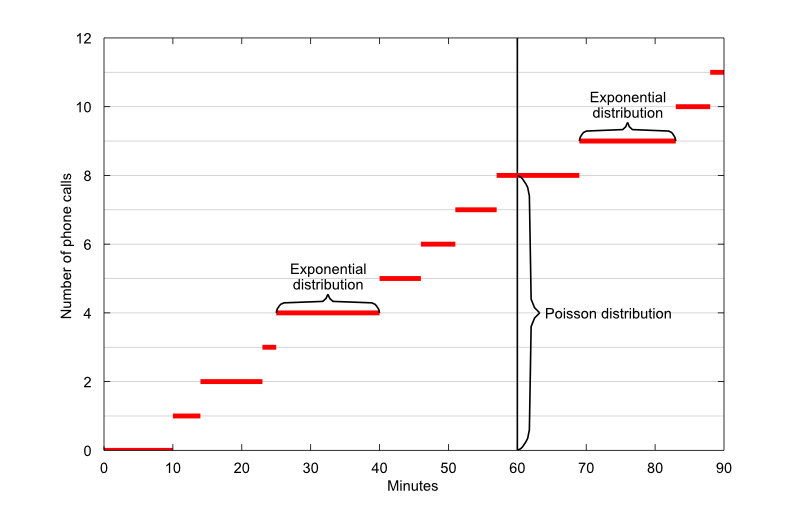
\includegraphics[scale=0.36]{pp.png}
 \par \centering{Everything about PP is shown in this figure.}
 \end{center}
}
 
 }
 
 
\frame{{Outline of this chapter 
\footnote{Section 3.4 and 3.5 in textbook are not covered in class.
All other materials in textbook for this chapter  are required}}
 \biz
 \item  Exponential \rv (review)
 \item  \po \rv  (review)
 \item  \pp
%\item Superposition and Thinning of a \pp
 \item  Compound \pp
 \eiz
 
 }
 
 
 \frame{{Exponential \rv:   ~~~ $ Exp(\lambda)$}
 
 \only<1>
 {
 A r.v. $X\geq 0$ with parameter $\lambda>0$ with the following pdf 
\[ p(x)= ? , x\geq 0. \]
The cdf is 
\[ F(x)=\p(X\leq x)=?, x\geq 0. \]
The expectation and variance is 
\[\e(X) =?, ~~\Var(X)= ? \]}
\only<2->
{
{\bf Definition}: A r.v. $X\geq 0$ with parameter $\lambda>0$ with the following pdf 
\[ p(x)=\lambda e^{-\lambda x}, x\geq 0. \]
The cdf is 
\[ F(x)=\p(X\leq x)=1-e^{-\lambda x}, x\geq 0. \]
The expectation and variance is 
\[\e(X) = \frac{1}{\lambda}, ~~\Var(X)=\frac{1}{\lambda^2}\]

 }
\only<3->{
\bigskip
Example 3.1 (page 60): the life time of machine is $Exp(\lambda)$  
}
 }
 
\frame{{Characteristic function and moment-generating function}
For a scalar random variable $X$,  the {\bf characteristic function} is defined as the expected value of $\e[e^{\ii tX]}$, where $\ii=\sqrt{-1}$ is the imaginary unit, and 
$t\in \Real$ is the argument of the characteristic function. If $X\sim Exp(\lambda)$, then
\[\varphi (t) := \e[e^{\ii t X}]= (1-\ii t \lambda^{-1})^{-1}, ~~t\in \Real.\]
\par
\bigskip 
\pause
The   {\bf moment-generating function} of $X\sim Exp(\lambda)$
$$M(\theta):= \e[e^{\theta X}]= (1- \theta \lambda^{-1})^{-1}, ~~~ -\infty <\theta< \lambda.$$
}
 
 \frame{
 {Memoryless Property (Thm 3.1)}
  
 \begin{theorem}
 Let $X$ be a continuous \rv\ taking values in $[0,+\infty)$.
 It has the memoryless property, i.e.,
 \[\p(X>t+s|X>s) = \p(X>t), \quad \forall s, t >0,\]
 {\it if and only if } 
 it is an $Exp(\lambda)$ for some $\lambda>0$.
 \end{theorem}

{\it Proof}:  page 61 (required). 
 }
 
 
 
 
 \frame{{\po \rv   $\sim Poi(\lambda)$}
 
 \only<1>
 {
 A r.v. $X\in S={0,1,2,3,\cdots}$ with parameter $\lambda>0$ with the following pdf 
 \footnote{it is called ``pmf" (probability mass function) in textbook for discrete \rv. }
\[ p(x)= ? , x\geq 0. \]
The cdf is 
\[ F(x)=\p(X\leq x)=?, x\geq 0. \]
The expectation and variance is 
\[\e(X) =?, ~~\Var(X)= ? \]}
\only<2->
{
{\bf Definition}: A r.v. $X\in S=\{0,1,2,3,\cdots\}$ with parameter $\lambda>0$ with the   pdf 
 
\[ p_k=\p(X=k)= e^{-\lambda}\frac{\lambda^k}{k!}. \]
 
The expectation and variance is 
\[\e(X) = {\lambda}, ~~\Var(X)= {\lambda}\]

 }
\only<3->{
\bigskip
Example 3.4 (page 69):   \po distribution as  the small probability limit of binomial distribution.
}
 }
 

\frame{{Moment-generating function}
The moment-generating function of  $X\sim Poi(\lambda)$ is 
\[ \boxed{
M(\theta) =\e [e^{\theta X}]= \exp\left( \lambda (e^\theta-1)\right )} , ~~\theta \in \Real.
\]
\begin{proof}
\[
\begin{split}
M(\theta)
&= \sum_{k=0}^\infty  e^{\theta k} e^{-\lambda}\frac{\lambda^k}{k!}
= e^{-\lambda} \sum_{k=0}^\infty  \frac{(e^{\theta }  \lambda)^k}{k!}\\
& = e^{-\lambda}  \exp(e^{\theta }  \lambda )\\
& =  \exp(e^{\theta }  \lambda -\lambda).
\end{split}
\]
\end{proof}

The characteristic function is 
\[\varphi (t) := \e[e^{\ii t X}]=  \exp\left( \lambda (e^{\ii t}-1)\right )  \]
}
\frame{
\begin{ex}  
(\footnotesize{\optional})
Suppose that $(Y_j)_{1\leq j\leq J}$ are independent  Poisson r.v.s
with $Y_j \sim Poi(\lambda_j)$ and $\set{a_j}$ are $J$ real numbers.  
Let $X:=\sum_{j=1}^J   a_j  Y_j  $ be the weighted average of $y_j$. 
Show that for  any $\theta\in \Real$, the Laplace transform of $X$ (i.e., the moment-generating function) is given by 
\[ \log   \e \left( e^{ \theta  X} \right) =  \sum_{j=1}^J  \left(e^{\theta a_j } -1 \right)\lambda_j
\]
\end{ex}
\pause
Proof:
\begin{align*}
  \e \left( e^{ \theta  X} \right) 
& = \e \left( e^{ \theta  \sum_{j=1}^J  y_j  a_j} \right) 
 = \e \left(  \Pi_{j=1}^J  e^{ \theta  y_j  a_j} \right) 
  =   \Pi_{j=1}^J  \e \left(  e^{ \theta  y_j  a_j} \right) 
 \end{align*}
 \begin{align*}
\log \left( \e \left( e^{ \theta  X} \right)  \right)
&   =   \sum_{j=1}^J  \log \left( \e \left(  e^{ \theta  y_j  a_j} \right)  \right)
   =   \sum_{j=1}^J  \log \left( \sum_{k=0}^\infty   e^{-\lambda_j} \frac{\lambda_j^k}{k!} \cdot  e^{ \theta  k  a_j} \right)   \\
   & =  \sum_{j=1}^J  \log \left(  e^{-\lambda_j}   \exp\left({\lambda_j e^{\theta a_j} } \right) \right)
   =\sum_{j=1}^J  \left(-\lambda_j + \lambda_j e^{\theta a_j}\right)
 \end{align*}

}


\frame{ \Large Poisson Process}


\frame{{Background of \pp}
\biz[<+->]
\item 
The   transitions from state to state are triggered by a stream  of events 
that occur at the sequence of times
\[ 0=S_0<S_1<S_2<\cdots<S_k<\cdots\]
 examples:  arrivals to a queuing system;
failures in a manufacturing system; biological stimuli in a neural system,
\item The successive inter-event time 
\[T_k := S_k - S_{k-1}\]   is a \rv\ in $[0,+\infty)$
\item The simplest model : \pp\ $N(t)$   ~~({\bf definition})
\biz
\item  Assume the inter-event time $\{T_k\} $ is    { iid  $Exp(\lambda)$ }. 
\item   The state space is $\ZZ$. The change of state is just to add  $``+1"$ to the old value:
 that is 
\[ N(S_k):=  N(S_k-)
\footnote{$N(t-)=\lim_{h\downarrow 0} N(t-h)$ 
is the left-limit. $\Real_+ = \{ x\in \Real: x\geq 0\}$} 
+1. \]  
\item 
$N(t)$ is thus the number of events arrived up to time $t$, i.e., within ${\color{blue}{(0,t]}}$.
by assuming  $N_0=0$.


\eiz 
\eiz

}

\frame{

Equivalently, the  \pp
  $\{N(t): t\in\Real_+)\}$ is defined as
\[
N(t) =\begin{cases}
 0 & ~~~\mbox{ if } 0\leq t < S_1 \\
 1 & ~~~\mbox{ if } S_1\leq t < S_2 \\
 2 & ~~~\mbox{ if } S_2 \leq t < S_3 \\
 \vdots &   
 \\
 k & ~~~\mbox{ if } S_k \leq t < S_{k+1} 
 \\
\vdots &   
 \end{cases}
\]
So, we have that 
\[ 
N(t)=\sum_{k=0}^\infty k\cdot1_{[S_k,S_{k+1})} (t)
=\sum_{k=1}^\infty 1_{[S_k,+\infty)} (t)
\]
and 
$\{N(t)\geq k\} \Longleftrightarrow \{ S_k \leq t  \}$.

}

\frame{
{A model of pure birth process}

Think of \pp\ as a special {\it counting process}  : count   ``the number  of customers to a queuing system
up to time $t$'', or a {\it pure birth process} (no death):  the species gives a descendant  with a rate $\lambda$.


\rule{\textwidth}{.4pt}

$T_n$ is the   time span  between arrivals of two successive  customers.
 
\pause
\biz
\item  iid assumption of $T_n$ is reasonable \footnote{the   process 
satisfying this condition  is in general called {\it renewal process}.}.
\item  Why $T_n$ is $Exp(\lambda)$? A ``microscopic'' model (short time asymptotics):

\eiz
\pause
Let $h$ be a small time step.  {\it Assume} during $(t, t+h]$, there is a probability ``$\lambda h$''
that one new customer will arrive, and ``$1-\lambda h$'' probability that no new customer will arrive
and this arrival event is {\bf independent}  of  the past information up to time $t$.
Then during time $(0,t)$ the probability of no arrival of new customer is 
\[\p (T_1>t) \approx  (1-\lambda h)^ {[t/h]} \to e^{-\lambda t},~~~\text{ as  }~h\to 0\]
where $ [t/h]$ is the integer part of $t/h$. This implies that 
$T_1$ is $Exp(\lambda)$.
\medskip 

This model is called a {\bf pure birth process.} We have   shown here the pure birth process
leads to an exponential distributed inter-arrival  time $T_i$.
}



\frame{{\pp:  $N(t)$}
$\lambda$ is called {\bf rate} {or {\bf intensity}} $=$ the prob. of exactly one arrival 
per unit time.
$$\boxed{ \lambda = \lim_{\delta t \to 0} \frac{1}{\delta t}\p( \text{ one arrival in } (t, t + \delta t]~ )  }$$

\par
 Denote the corresponding \pp\ $N(t)$  as $PP(\lambda)$.
 
  
 \begin{center}
 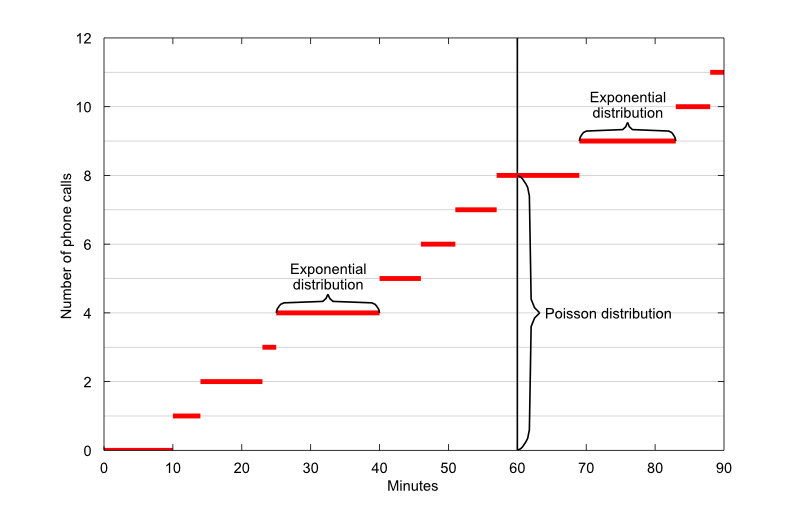
\includegraphics[scale=0.33]{pp.png}
 \end{center}

}




\frame{{Why has the name ``Poisson'' process?}
 

\begin {theorem}[Thm 3.6, 3.7 (p71)]

Let $\{N(t)\}$ be a $PP(\lambda)$. 

\biz

\item It is a Markov process: that is 
\[  \p(N(t+s) =k | N(s)=j, N(u), 0\leq u\leq s)
=  \p(N(t+s) =k | N(s)=j)\]

\item 
For a given $t$, 
$N(t)\sim Poi(\lambda t)$. That is 
\[ \p(N(t)=k)=e^{-\lambda t}\frac{\lambda^k t^k}{k!}
\]
\eiz
\end{theorem}
}

\frame{ {sketch of proof in textbook}

 \begin{proof}
First, note that 
$\{N(t)\geq k\} = \{ S_k \leq t  \}$ because
\biz
\item
If $N(t)\geq k$, then 
there exists $n\geq k$ such that $S_n \leq t$.
Noting by definition   that $S_n \geq S_k$  for all $n\geq k$.
So, we have $S_k \leq t$.
\item 
If $S_k \leq t$, then  $k \in \{n\geq 0:  S_n\leq t\}$ and 
$k \leq N(t)$ by definition.
\eiz
Second, 
$\p(N(t)\geq k)=\p(S_k \leq t) = \p(\sum_{i=0}^k T_i \leq t)
$. The sum of $k$ iid r.v.s $\{T_i\}\sim  Exp(\lambda)$ follows  the Erlang distribution
with CDF $F(x)=1-\sum_{r=0}^{k-1} e^{-\lambda x} (\lambda x)^r/ r!$  (Eqn. (3.9), p62, textbook).
\\
Then the conclusion follows after some calculations 
for $\p(N(t)= k)=\p(N(t)\geq k)-\p(N(t)\geq k+1)$
\end{proof}

}



\frame{ {An alternative  (and easy) proof
\footnote{\url{https://www.netlab.tkk.fi/opetus/s38143/luennot/E_poisson.pdf}}
}
\framesubtitle{this proof can be generalized to inhomogeneous \pp\ where $\lambda$ is a function of time}
\vskip -8pt
We  start from the pure birth process  
and prove the theorem (only part (ii)) by computing the moment-generating function  of $N(t)$:  
\[ \mathcal{G} (t, \theta) := \e [e^{\theta N(t)}]\]
Note that $Poi(t \lambda)$'s momentum generating function is  $M_t(\theta)= \exp\left(  t \lambda (e^\theta-1)\right )$.
So we just need to show   $\mathcal{G}(t, \theta) =M_t(\theta)$, equivalently $\log \mathcal{G} = t \lambda (e^\theta-1)$. \pause
Introduce the number of arrivals during time interval $(s, t]$ for $0\leq s<t$: 
\[ N(s,t) := N(t) -N(s)\]
Then 
$\displaystyle \dot{\mathcal{G}}(t,\theta)=\lim_{h\to0 } \frac{\mathcal{G}(t+h,\theta)-\mathcal{G}(t,\theta)}{h}
=\lim_{h\to0 }   {h}^{-1}   \e \left [e^{\theta\left (N(0,t)+N(t,t+h)   \right)  } -  e^{\theta   N(0,t)   } \right] $  \pause
Note that  by the independence between $(0,t]$ and $(t,t+h]$, we have
\[
\begin{split}
& \e \left [e^{\theta\left (N(0,t)+N(t,t+h)   \right)  } -  e^{\theta   N(0,t)   } \right]
  = 
  \e \left [ e^{\theta N(0,t) } \left (   e^{\theta   N(t,t+h) }  -1 \right) \right] 
  \\
  = &  \e \left [ e^{\theta N(0,t) }\right ]\e \left[   e^{\theta   N(t,t+h) }-1 \right] = \mathcal{G}(t,\theta) 
 \left[    ( e^{\theta}-1 ) h \lambda + (1-1)\times (1-\lambda h ) + O(h^2) \right]\\
  \end{split}
\] \pause
So, we have ODE $\dot {\mathcal{G}}(t,\theta) = \mathcal{G} (t,\theta) (e^{\theta}-1) \lambda $,
 i.e., $\frac{d}{dt}{\log \mathcal{G}} =  \lambda (e^\theta-1)$. Since $\mathcal{G}(0,\theta)=1$,
 the conclusion is obtained.
}

\frame{ 
{Properties of 
{\pp}}


Let $\{N(t)\}$ be a $PP(\lambda)$.
\ben [<+->]
\item  
It is a Markov process.
\item
With probability 1, the sample path  $N(t)$ is right-continuous with left limits \footnote{This property is  abbreviated as ``LLRC'' and 
also popularly  called 
{C\`{a}dl\`{a}g} in French language, meaning "continue \`{a} droite, limite \`{a} gauche".}
\item
$N(t) = \max\{n\geq 0:  S_n \leq t\}, ~~t\geq 0.$
\item $\{N(t)\geq k\} = \{ S_k \leq t  \},   t\in\Real_+, k=1,2,\ldots.$
).
\item Reconstruction of  the jump time :
$ S_n =\inf\{t\in \Real_+ : N_t =n\}, n\geq 1.$

\item  $N(t+s)-N(t)$ means the number of arrival events during time period $(t,t+s]$.

 \item {\bf 
Independence of increments}: for all $0\leq t_0 < t_1 <\cdots<t_n$ and $n\geq 1$, the increments
$N_{t_1} -N_{t_0},\ldots, N_{t_n} -N_{t_{n-1}}$ 
over the disjoint time intervals $(t_0,t_1], (t_1,t_2], \ldots, (t_{n-2},t_{n-1}],
 (t_{n-1},t_n]$
are  mutually  independent random variables.
In particular, $N_t=N_t-N_0$ is independent of $N_{t+s}-N_t$ for $\forall s, t >0$.

\item {\bf Stationarity of increments}:  $N_{t+h} - N_{s+h}$ has the same distribution as
$N_t -N_s$ for all $ h>0 $ and $0\leq s\leq t$. This is
\[\p(N_{t+h} - N_{s+h}   =k) = \p(N_t -N_s=k) \]

\een 



}

\frame{ {Review of the increment for DTMC random walk (assignment 1)}
For the above independent and stationary increments,  the  Random Walk 
$\set{X_n}=\sum_{i=0}^n Z_i$ also has these two properties:
\biz
\item   $X_{n+k}-X_{n}$ is independent from $X_{n+k+m}-X_{n+k+l}$ for $m>l>0$.
\item   $X_{n+k}-X_{n}$  and  $X_{n+m+k}-X_{n+m}$  have the same distribution as 
$\sum_{i=1}^k {Z_i}$ 
\eiz  

\pause
\vfill
Recall the assignment   of calculating the auto-covariance function 
\[\begin{split}
\Cov(X_{m+n}, X_m)&=
\e\left [\left ((X_{m}  -m\mu) + \sum_{i=m+1}^{m+n} (Z_i - \mu)\right)(X_m - m\mu)\right] \\
&=\Var(X_m) + \sum_{i=m+1}^{m+n} \e\left[  (Z_i - \mu)(X_m - m\mu)\right] 
\\
&=
\Var(X_m) + \sum_{i=m+1}^{m+n}  \e (Z_i - \mu) \cdot \e (X_m - m\mu) 
\\
&=\Var(X_m)\\
 &= 4mpq  
\end{split}
\]
Here we used the independent increment property ! We shall see this application again for \pp.
 }

\frame{
{\bf {corollary}
}
\biz
\item[\snum{1}] $\e(N(t))=\lambda t$ , $\Var(N(t))=\lambda t$,
$\e(N(t))^2 = \lambda t + \lambda^2 t^2$.
\item[\snum{2}]  stationary increment 
\[N(t+s)-N(s) \sim N(t)-N(0) \sim Poi(\lambda t)\]
\item[\snum{3}]  covariance function 
\[
\begin{split}
\Cov(N(t+s),N(s))&= \e\big [(N(t+s)-(t+s)\lambda)\cdot (N(s) -s \lambda) \big]
=\lambda s\\
\Cov(N(t),N(s))&= \lambda (s  \wedge t)
\end{split}
\]
\eiz

}



\frame{{ Exercise}
\only<1>{
 $N(t)\sim PP(\lambda)$. $S_n $ is the $n$th jump time.
Let $t_i=i$ for $i=1,2,3,4$.

\ben
\item  What is the expected number of arrival customers at time $t_4$?
\item  What is the probably that there are no arrivals from $t_1$ to $t_3$?
\item What is the probably that there are two arrivals  from $t_1$ to $t_3$,
and for these two events, one arrives before $t_2$ and the other arrives after $t_2$ ?
\item What is the probably that there are two arrivals  from $t_1$ to $t_4$
among which  one arrives before $t_3$ and the other arrives after $t_2$ ?
\item $\p(N(t_3) =5|N(t_1) =1)=?$
\item $\e(N(t_2)N(t_1)) = ? $
\item $\e[N(t_2) | S_1 >t_1]  = ?$
\een}

\only<2-|handout:0>{
\vskip -12pt
\ben[<+->]
\item  $\e(N(t_4))=\lambda t_4=4\lambda$
\item  $\p(N(t_3)-N(t_1)=0)=\p(N(t_3-t_1)=0)=e^{-\lambda(t_3-t_1)}=e^{-2\lambda}$.


\item   
 \[
\begin{split}
&\p(N(t_2)-N(t_1)=1, N(t_3)-N(t_2)=1) \\
=&\p(N(t_2)-N(t_1)=1) \p( N(t_3)-N(t_2)=1) \\
=&e^{-\lambda (t_2-t_1)} \lambda (t_2-t_1) 
e^{-\lambda (t_3-t_2)} \lambda (t_3-t_2)=
 \lambda^2 e^{-2\lambda }
 \end{split}
\]


\item   
  We need discuss all possible cases in the following table.
  The answer is the sum of the last columns :
 $3 \lambda^2 e^{-2\lambda} + \lambda^2 e^{-\lambda}/ 2$ 

\begin{center}
\footnotesize \begin{tabular}{|ccc|c|}
\hline 
$(t_1, t_2]$ & $(t_2, t_3]$ & $(t_3, t_4]$ & \mbox{prob} \\
\hline
 1 & 1 & 0 & $\lambda^2 e^{-2\lambda}$\\
 0 & 2 & 0 &  $\lambda^2 e^{-\lambda}/ 2$\\
 0 & 1 &  1  & $\lambda^2 e^{-2\lambda}$\\
 1 & 0 & 1  & $\lambda^2 e^{-2\lambda}$
\\ \hline
\end{tabular}
\end{center}



\item $\p(N(t_3) =5|N(t_1) =1)=
\p(N(t_3)-N(t_1) =4|N(t_1) =1)
=\p(N(t_3-t_1) =4) = \frac{\lambda^4 (t_3-t_1)^4 }{4!} e^{-\lambda(t_3-t_1)}
=\frac{ 2\lambda^4  }{3} e^{-2\lambda}
$




\item $\e(N(t_2)N(t_1)) = 
\e[(N(t_2)-N(t_1) ) N(t_1)] + \e(N(t_1)^2) 
=\e(N(t_2)-N(t_1) ) \e(N(t_1))+ \e(N(t_1)^2) =
2\lambda^2+\lambda$
\item $\e[N(t_2) | S_1 >t_1]  = 
\e[N(t_2) | N(t_1) < 1 ]
= \e[N(t_2) | N(t_1) =0 ]
=\e[N(t_2-t_1) ] = \lambda 
 $
\een}

}
 
 
 \frame{{Conditional distribution of jump times 
 \footnote{Theorem 2.3.1 p.67 in {\it Stochastic Processes} by Ross, S.M. 
 Wiley,  2nd Edition,1996. } }
 \begin{theorem}
 Fix $T$ and  condition the PP $N(t)$ to have 
 $K$ jumps in this interval $[0,T]$.
 Then, regardless of the Poisson rate $\lambda$,
 the jump times $\{S_k:k=1,\cdots,K\}$ are distributed as 
 $K$ i.i.d. uniform $[0,T]$ r.v.s. 
 (actually as their  order statistics since
 you need to rearrange these 
 uniform r.v.s in increasing order.) That is 
 \[ (S_1,S_2,\cdots, S_K)\sim 
 (X_{(1)}, \cdots,(X_{(K)} )
 \]
 where $X_{(1)}\leq \cdots\leq X_{(K)} $
is  the {\bf  order statistics} of  $\set{X_k:k=1,\cdots,K}$
\footnote{$X_{(i)}$ is the $i$-th smallest value among $(X_k:k=1,\cdots,K)$.}
and $X_k$ are i.i.d. uniform r.v.s in $[0,T]$.
 \end{theorem}
 \pause
 Note that  the joint pdf of   the uniform order statistics 
 is   \[f(s_1,s_2,\cdots,s_K) \equiv \frac{K!}{T^K}.\]
 
  For $K=1$, the proof is an exercise.

 }

\frame
{
\begin{proof}
We shall compute the conditional density function of 
$S_1,S_2,\cdots,S_K$ given that $N(T)=K$.
Let $0<t_1<t_2\cdots<t_K\leq  T$ and let 
$h_i$ be small enough so that $(t_i-h_i/2 , t_{i}+h_i/2]$
has no overlap for any $ i = 1,\cdots,K$.
Now 
\[
\begin{split}
&\cPr{ S_i \in (t_i-h_i/2, t_i+h_i/2], i=1,2,\cdots,K }{N(t)=K}\\
&= \frac{1}{\p(N(t)=K)}\times
\p( \mbox{exactly one event in }   (t_i-h_i/2, t_i+h_i/2] ,, i=1,2,\cdots,K  
\\
& ~~\qquad \qquad\qquad~  \mbox{and  \hb{no events elsewhere} }) \\
&= \frac{   \Pi_{i=1}^K (\lambda h_i e^{-\lambda h_i})   \times  \hb{e^{-\lambda (T -\sum_i h_i)}}}
{e^{-\lambda T} (\lambda T)^K / K!}\\
&= \frac{K!}{T^K} \Pi_{i=1}^K    h_i
\end{split}
\]
By letting $h_i\to 0$, we obtain that the conditional {\it density} is
\[ f(t_1,\cdots, t_K) =\frac{K!}{T^K}, ~~0<t_1<\cdots<t_K<T. \]

\end{proof}


}

\frame{
{Compound \pp   (cPP)  }
At each arrival time $S_n$, the jump size 
is also random.   
 \begin{center}
 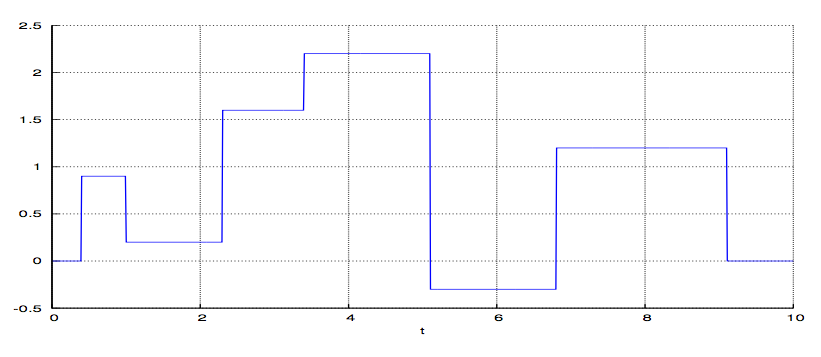
\includegraphics[scale=0.33]{CPP.png}\\
A sample path of compound PP.
 \end{center}

}


\frame{
{Compound \pp   (cPP)  }
 
\medskip

\begin{definition}
At each jump time, the jump size is from iid r.v. $Z_n$ following the distribution  $\nu$.
And $\set{Z_n}$ is also independent of the PP. Define 
\[ C(t) =C(0)+ \sum_{n=1}^{N(t)} Z_n
=C(0)+ \sum_{k=1}^\infty Z_k 1_{\set{S_k\leq t}}\]
\end{definition}
{\footnotesize( $\sum_{n=1}^0 :=0$). We assume $C(0)=0$. $Z_n\equiv 1$ gives the standard \pp.}
  



\[
C(t) =\begin{cases}
 0 & ~~~\mbox{ if } 0\leq t < S_1 \\
 Z_1 & ~~~\mbox{ if } S_1\leq t < S_2 \\
 Z_1+Z_2 & ~~~\mbox{ if } S_2 \leq t < S_3 \\
 \vdots &   
 \\
 \sum_{n=1}^k Z_n & ~~~\mbox{ if } S_k \leq t < S_{k+1} 
 \\
\vdots &   
 \end{cases}
\]


}

\frame{{Characteristic function of compound Poisson process}
$Z_1,Z_2,\cdots,Z_n$, are iid r.v.  on $\Real$ with distribution  $\nu(z)dz$.
Denote the characteristic function  of $Z_1$ as 
\[ g(\alpha):=\e e^{\ii\alpha Z_1}=\int_{\Real}  e^{\ii z\alpha}   \nu(z) dz ,
~~  \ii:=\sqrt{-1}.\]
 Then we can  compute the  {characteristic function}
of the increment $C_t-C_s$ for any $0\leq s<t$
as follows. 
 \begin{theorem}
 \[\e \left [ \exp ( i \alpha (C_t - C_s) \right] 
= \exp 
\left(
\lambda (t-s) \int_{\Real}  (e^{ i z\alpha} - 1) \nu(z) dz
\right)=e^{ 
\lambda (t-s)  (g(\alpha)-1) },    \forall \alpha \in \Real
\]
\end{theorem}
 }

\frame{

\begin{proof}
{\small
(step 1): definition;
(step 2): law of total prob. and indpt. of $N$ and $Z$;
(step 3): iid of $Z_k$ and indpt. increment of $N$.}
\vskip -2em
\begin{align*}
&\e \left [ \exp ( i \alpha (C_t - C_s) \right] 
=\e \left [ \exp \left( i \alpha \sum_{k=N_s+1}^{N_t} Z_k \right )\right]
~~\because ~\mbox{ law. of total. prob.}
\\ 
&= \sum_{n=0}^\infty 
\sum_{m=0}^\infty
\e \left [ \exp \left( i \alpha \sum_{k=m+1}^{m+n} Z_k \right) \right]
\p (N_s=m, N_t-N_s=n)
\\
&= \sum_{n=0}^\infty 
\sum_{m=0}^\infty
\e \left [ \exp \left( i \alpha \sum_{k=1}^{n} Z_k \right) \right]
\p (N_s=m) \p( N_t-N_s=n)
\\
&= \sum_{n=0}^\infty 
\e \left [ \exp \left( i \alpha \sum_{k=1}^{n} Z_k \right) \right]
\p( N_t-N_s=n)
\left ( \sum_{m=0}^\infty
\p (N_s=m) \right) 
\\
&= \sum_{n=0}^\infty 
 \left(\e\left [  \exp \left( i \alpha  Z_1 \right) \right]\right)^n
 \times
e^{-\lambda(t-s)} \frac{\lambda^n (t-s)^n}{n !}
\times 1
\\
&=\exp 
\left( \lambda(t-s) \e \left [  \exp \left( i \alpha  Z_1 \right) \right]
   \right)
   e^{-\lambda(t-s)}\\
   &=\exp 
\bigg( \lambda(t-s) \left( \e   [  \exp \left( i \alpha  Z_1 \right)  ] -1\right)
   \bigg)
   \\
   &=
   \exp 
\left(
\lambda (t-s) \int_{\Real}  (e^{ i z\alpha} - 1) \nu(z) dz
\right)
   \end{align*}
\end{proof}
}

\frame{{Examples}
\biz
 
\item  If  $Z(\omega)\equiv 1$, then $C_t$ is just the standard \pp, $PP(\lambda)$.
Now $\nu(z)  = \delta(z-1)$  and $ \e Z_1=\e Z_1^2=1$,
$g(\alpha)=e^{\ii  \alpha }$.
We calculate the characteristic function by the above formula
and obtain that 
\[\e \left [ \exp ( i \alpha (C_t - C_s) \right] 
= \exp 
\left(
\lambda (t-s)  (e^{ i \alpha} - 1)  
\right).
\]
Actually, if a continuous-time stochastic process 
has the same characteristic function as this,
then it has the same distribution as the  \pp\ $PP(\lambda)$.

\item
If $(Z_i)$ is   a sequence of Bernoulli
trials with parameter $p$: 
$\p(Z_1=1)=p$ and $\p(Z_1=0)=q$.
Show that the compound \pp\ is 
actually a \pp\ with rate $p\lambda$.

\pause
We calculate $g(\alpha)=e^{\ii\alpha}p + (1-p)$.
Then 
 \[
 \e \left [ \exp ( i \alpha (C_t - C_s) \right] 
=  \exp \big(
\lambda (t-s)  (e^{\ii\alpha}p -p) \big)
=\exp \left(
p \lambda (t-s)  (e^{\ii\alpha} -1) \right)
\]
This means that $(C_t)$ is a $PP(p\lambda)$.
\eiz
}

\frame{{Applications}

 We can derive the  mean and variance of $C(t)$ from the characteristic function.
(Thm 3.11 in textbook uses alternative proof by considering the 
iid random sum of r.v.s)
 Set $s=0$ and $C_0=0$ and note that $g'(0)=\ii \e Z_1$ and 
 $g''(0)=-\e (Z_1)^2$

 

\biz 
\item 
\[\e[C_t] = -\ii \frac{d}{d\alpha} \e [ e^{\ii \alpha C_t}] \vert_{\alpha=0}
=-\ii \lambda t g'(0)=\lambda t \int_\Real z\nu(z)dz = \lambda t\cdot \e Z_1\]
So, after subtracted by the compensator $\lambda   (\e Z_1) t$,
the new process 
$ C_t - (\lambda\cdot   \e Z_1) t $
is called ``compensated'' compound Poisson process, 
because is  has zero mean (actually it is a martingale). 
\item  \[\e[C_t^2] = - \frac{d^2}{d \alpha^2} \e [ e^{\ii\alpha C_t}] \vert_{\alpha=0}
= - \lambda t ( g''(0) + \lambda t(g'(0))^2 )
= \lambda t\big (   \e Z_1^2  +  \lambda t(\e Z_1 )^2 \big) 
\]
\item The variance is thus 
$\Var[C_t]=\lambda t \cdot \e Z_1^2$.
\item  $(C_t)$ has stationary increment  
because  the characteristic function for 
the increment $C_t-C_s $ only  depends on 
the difference $t-s$.

\item  $(C_t)$ has independent increment  
because (verify by yourself)
\[\e \left[ \Pi_{k=1}^n 
e^{i \alpha_k (C_{t_k}- C_{t_{k-1}})}\right]
= \Pi_{k=1}^n 
\e \left[
e^{i \alpha_k (C_{t_k}- C_{t_{k-1}})}\right]
\]

\eiz
}

\frame{
\biz
\item The covariance  function
\[
\begin{split}
&\Cov(C_{t+s}, C_s) \\
=& \e [ (C_{t+s}-\e C_{t+s})( C_s - \e C_s)]\\
=&\e [C_{t+s}C_s] - (\e C_{t+s} \cdot \e C_s)\\
=&\e [(C_{t+s}-C_s)C_s] +\e  (C_{s})^2  - (\e C_{t+s} \cdot \e C_s)\\
=&\e [(C_{t+s}-C_s)] \cdot \e [C_s] +\e  (C_{s})^2  - \e C_{t+s} \cdot \e C_s \\
=& - (\e C_s)^2 +  \e  (C_{s})^2 \\
= & \Var (C_s) \\
=& (\lambda \cdot \e Z_1^2 )s\\
\therefore~~ \Cov(C_{t}, C_s) &= (\lambda \cdot \e Z_1^2 ) ( s \wedge t).
\end{split}
\]



\item Markov property : $(C_t)$ is a continuous-time Markov process.
\item Restaurant Arrival Process (Example 3.9)
\eiz
}
 
\frame
{
{\hw}

\biz

\item Prove Thm3.3, Thm 3.5 in textbook
(do not read the proof in textbook first. try independently )

%\item For each $k\geq 0$, fine a number $\alpha_k$ such that  $\lim_{h\downarrow 0} \frac{\p(N(h)=k)}{h^{\alpha_k}}$ 
%is a positive constant.
%By this we can have $\p(N(h)=k) \sim O(h^{\alpha_k})$ for short time $h$. 

 


\item  Exercise 3.9, 3.10, 3.17, 3.19, 3.20,  3.25 (CONCEPTUAL PROBLEMS, page 79)
\item Exercise 3.2,  3.3, 3.29, 3.30 (COMPUTATIONAL PROBLEMS, page  80)

\item 
Let $N$ be a Poisson process with parameter $\lambda$.
Let $U_t$ denote the time of the first jump
{\it after}  time t. (In particular, $U_0$ = $S_1$.)
 Calculate the probability density function of $U_t$.


\eiz

 }
 
 \frame{
\biz 
\item 
Let $N(t)$ be the number of arrival customers
and assume $\{N(t)\}$ is  a \pp with rate $ \lambda$. $S_n$ is the $n$th jump time.
Let  $t_i=i$ for $i=1,2,3,4$.
\ben
\item  What is the expected number of arrival customers at time $t_4$?
\item  What is the probably that there are no arrivals from $t_1$ to $t_3$?
\item What is the probably that there are two arrivals  from $t_1$ to $t_3$
and one arrives before $t_2$ and the other arrives after $t_2$ ?
\item $\p(N(t_3) =5|N(t_1) =1)=?$
\item $\e(N(t_2)N(t_1)) = ? $
\item  $\e [N(t_1)N(t_4)(N(t_3) -N(t_2))] = ?$
\item $\e[N(t_2) | S_1 >t_1] $
\item   $\e[N(t_2) | S_2 >t_1] $ 
\een
\eiz

 }

\end{document}
